\chapter[Datasets details]{Some details on the datasets used}
\section{TCGA}

	\begin{table}[htbp]
	    \sisetup{detect-mode}
	    \centering
	    \caption{Cancer repartition in the \glsfmtshort{tcga} dataset.}\label{tab:data_cancer_tcga}
	    \begin{tblr}{
	        colspec={
	                Q[r,m]
	                Q[si={table-format=4,table-number-alignment=center},wd=2.4cm,r]
	                Q[r,m]
	                Q[si={table-format=4,table-number-alignment=center},wd=2.4cm,r]
	            },%
	        row{2-Z} = {font=\small},%
	        row{1} = {guard, c,m, font=\bfseries},%
	        hline{1,Z} = {2pt},%
	                hline{2} = {1pt},%
	            }
	        Cancer & {Number              \\of samples} & Cancer & {Number\\of samples} \\
	        Normal & 1354    & PRAD & 499 \\
	        BRCA   & 1106    & SKCM & 474 \\
	        OV     & 620     & COAD & 463 \\
	        LUAD   & 583     & STAD & 443 \\
	        UCEC   & 549     & BLCA & 413 \\
	        KIRC   & 539     & LIHC & 380 \\
	        LGG    & 534     & CESC & 309 \\
	        HNSC   & 530     & KIRP & 292 \\
	        THCA   & 515     & SARC & 266 \\
	        LUSC   & 505     &      &     \\
	    \end{tblr}
	\end{table}

	\begin{table}[htbp]
	    \sisetup{detect-mode}
	    \centering
	    \caption{Number of features in each omics for the \glsfmtshort{tcga} dataset.}\label{tab:data_features_tcga}
	    \begin{tblr}{
	        colspec={
	                Q[r,m]
	                Q[si={table-format=5,table-number-alignment=center},wd=2.5cm,r]
	            },%
	        row{2-Z} = {font=\small},%
	        row{1} = {guard, c,m, font=\bfseries},%
	        hline{1,Z} = {2pt},%
	                hline{2} = {1pt},%
	            }
	        Omics           & {Number \\of features} \\
	        CNV             & 60226   \\
	        mRNA            & 56902   \\
	        mRNA coding     & 19887   \\
	        mRNA non coding & 33883   \\
	        miRNA           & 1621    \\
	        DNAm            & 22596   \\
	        DNAm genes      & 14197   \\
	        Proteins        & 454     \\
	    \end{tblr}
	\end{table}

	\begin{figure}[htbp]
	    \centering
	    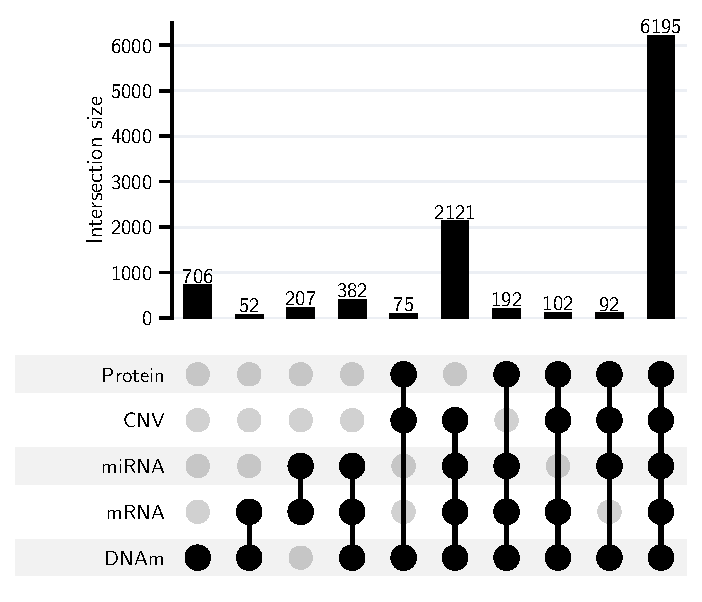
\includegraphics{size_per_omics_comb.pdf}
	    \caption{Number of samples available with various omics combination in \glsfmtshort{tcga}.}\label{fig:omics_comb_sizes}
	\end{figure}

	\newpage
\section{CCLE}

	\begin{table}[htbp]
	    \sisetup{detect-mode}
	    \centering
	    \caption{Cancer repartition in the \glsfmtshort{ccle} dataset.}\label{tab:data_cancer_ccle}
	    \begin{tblr}{
	        colspec={
	                Q[r,m]
	                Q[si={table-format=2,table-number-alignment=center},wd=2.4cm,r]
	                Q[r,m]
	                Q[si={table-format=2,table-number-alignment=center},wd=2.4cm,r]
	            },%
	        row{2-Z} = {font=\small},%
	        row{1} = {guard, c,m, font=\bfseries},%
	        hline{1,Z} = {2pt},%
	                hline{2} = {1pt},%
	            }
	        Cancer & {Number             \\of samples} & Cancer & {Number\\of samples} \\
	        LUAD   & 78      & KIRC & 39 \\
	        {COAD                        \\READ}   & 64    & SARC & 38 \\
	        SKCM   & 59      & LAML & 38 \\
	        SCLC   & 53      & STAD & 38 \\
	        BRCA   & 53      & GBM  & 34 \\
	        OV     & 50      & HNSC & 34 \\
	        PAAD   & 43      & ALL  & 33 \\
	        DLBC   & 40      & MM   & 30 \\
	    \end{tblr}
	\end{table}

	\begin{table}[htbp]
	    \sisetup{detect-mode}
	    \centering
	    \caption{Number of features in each omics for the \glsfmtshort{ccle} dataset.}\label{tab:data_features_ccle}
	    \begin{tblr}{
	        colspec={
	                Q[r,m]
	                Q[si={table-format=5,table-number-alignment=center},wd=2.5cm,r]
	            },%
	        row{2-Z} = {font=\small},%
	        row{1} = {guard, c,m, font=\bfseries},%
	        hline{1,Z} = {2pt},%
	                hline{2} = {1pt},%
	            }
	        Omics        & {Number \\of features} \\
	        CNV          & 23316   \\
	        mRNA         & 55248   \\
	        miRNA        & 734     \\
	        DNAm         & 19096   \\
	        Metabolomics & 225     \\
	        Protens      & 214     \\
	    \end{tblr}
	\end{table}

	\begin{figure}[htbp]
	    \centering
	    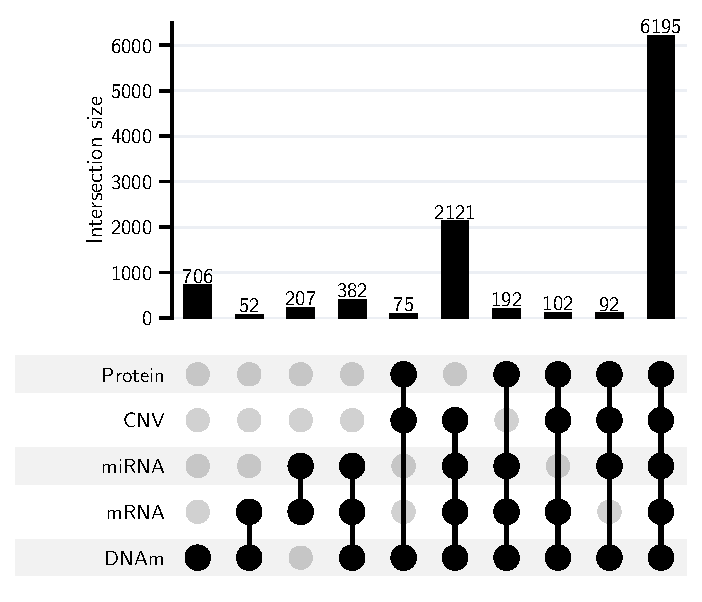
\includegraphics{size_per_omics_comb.pdf}
	    \caption{Number of samples available with various omics combination in \glsfmtshort{ccle}.}\label{fig:omics_comb_sizes_ccle}
	\end{figure}
